\documentclass[letterpaper, 12 pt, conference]{article}
\usepackage{setspace}
\usepackage{listings}
\usepackage{color}
\usepackage{float}
\usepackage{graphicx}
\usepackage{hyperref}
\usepackage[utf8]{inputenc}
\usepackage[english]{babel}

\definecolor{dkgreen}{rgb}{0,0.6,0}
\definecolor{gray}{rgb}{0.5,0.5,0.5}
\definecolor{mauve}{rgb}{0.58,0,0.82}

\lstset{frame=tb,
  language=R,
  aboveskip=3mm,
  belowskip=3mm,
  showstringspaces=false,
  columns=flexible,
  basicstyle={\small\ttfamily},
  numbers=none,
  numberstyle=\tiny\color{gray},
  keywordstyle=\color{blue},
  commentstyle=\color{dkgreen},
  stringstyle=\color{mauve},
  breaklines=true,
  breakatwhitespace=true,
  tabsize=3
}

\setlength{\parindent}{4em}
\setlength{\parskip}{1em}

\title{Term Project}
\author{Alan Wu, Dongyu  Chen, Rishabh Manu, Joshua Winter}
\date{March 2021}

\begin{document}

\maketitle

\section{Part A}
\begin{enumerate}
    \item 
    \textbf{Title: Reactivation of Previous Experiences in a Working Memory Task} 
     \\ 
     \textbf{Authors: Gi-Yeul Bae, from Arizona State University and Steven J. Luck, from University of California, Davis }
    \\
    \textbf{Link:} 
    \url{https://www.ncbi.nlm.nih.gov/pmc/articles/PMC6472175/}
    \\
    \textbf{Team Member: } Alan Wu
    \\\\
    The paper of concern researches whether recent experiences irrelevant to the current task have any role or effect on the current task; is the previous task representation reactivated when the current task is presented? For each trial in the experiment, participants were presented with a teardrop that was oriented in 1 of 16 different directions. After a short delay, the participant was asked to configure a new teardrop to the previously shown orientation from memory. It was found that in successive trials, previous trial orientation could be decoded from the current trial electroencephalogram (EEG). This was possible because previous trial information was reactivated, and therefore detectable. The results of the study show that recent experiences that are not relevant to the current task can influence processing of the current task. 

I will focus on the paper's analysis of the behavioral response in each trial, where reported orientation of the teardrop was measured in comparison to the sample teardrop; positive values indicated clockwise errors while negative values indicated counterclockwise errors. The null hypothesis claims that previous trial teardrop orientation has no influence on current trial orientation error. The magnitude of serial dependence is based on a function defined by the first derivative of a Gaussian: 

$$E = \alpha \times wx \times ce^{-(wx)^2} + \beta $$

We will focus on alpha, the amplitude of the peak of the curve. A high magnitude alpha value would indicate serial dependence (the previous trial orientation has influenced current trial orientation). Conversely, $\alpha = 0$ would indicate no effect from the previous trial. The results of a one-sample t test indicated the amplitude of the function: 
\begin{equation}
(15) = −9.731, p = 7.143*10^{-8}
\end{equation}
It appears that the p value is incredibly low, which suggests that previous trial orientation likely does influence the current task. However, this low p value could be due to the result of a very high number of trials, as 640 trials (40 for each of the 16 orientations) were conducted for each of the 32 total college students. Instead, a confidence interval could be introduced, which would give a range of values $\alpha$ can be expected to be between. $\alpha$ values within a range much greater than or less than zero (high magnitude) would be consistent with the paper's findings. Using a confidence interval would also be more informative, as it specifies not only how great the magnitude is (how far away from 0, again, with 0 meaning no relation between previous and current trials), but also how accurate the interval is; this would benefit the study as it appears a large sample size was used given the sheer number of trials. 

    
    \item
     \textbf{Title: } Longitudinal variability of time-location/activity patterns of population at different ages: a longitudinal study in California
     \\ 
     \textbf{Reasearchers: } Xiangmei Wu, Deborah H Bennett, Kiyoung Lee, Diana L Cassady, Beate Ritz, and Irva Hertz-Picciotto
    \\
    \textbf{Link: } 
    \url{https://ehjournal.biomedcentral.com/articles/10.1186/1476-069X-10-80}
    \\
    \textbf{Team Member: } Joshua Winter
    \\\\
    In this paper, researchers examine the activity patterns of a California population in order to provide information for future exposure modeling of toxic environmental compounds. This longitudinal study randomly selected 186 households in Northern California containing at least one child less than 8 years old and 64 households in Southern Central California containing adults older than 55 years old. Conducted from October 2007 through September 2009, participating households recorded their activity, time, and location at 30 various “microenvironments” and activities including using a stove, at school, at transit, at a restaurant, in an office building, sleeping, and doing a general vigorous activity. The participants recorded their data on a monthly basis via an internet survey in which they uploaded a 24-hour recall of their activities the day before.
     \\\\
     For data analysis, the study compared the activity patterns observed with the following covariates: day-type (weekday vs. weekend), season, time, sex, and age. The researchers created two tables to denote the variation of time in selected microenvironments as well as the variation of activities collected from the questionnaires. These tables omitted results where $p < .05$ (the study had $\alpha$ = .05) to only show results where there was a statistically significant relationship between a covariate and the activity pattern of the sample group. Some of the results they had found based upon significance testing were an increasing trend in gym visits as the season got cooler, female children tended to spend more time in school than their male counterparts, a decreasing trend in computer use on weekends from weekdays in adults, and an increasing trend to visit food stores in warmer seasons.
    \\\\
     This study limited its scope of whether there was a statistically significant relationship between the activity patterns and the covariates to a discretely binary decision through the use of p-values. Creating future exposure models and policies off of this data may lead to faulty decision-making since some relationships may be falsely interpreted. It is difficult to say whether certain relationships not included in the results table are insignificant or that those that were included truly are significant since we could have values like .053 that wouldn’t be included and values like .047 that would be included. From our relatively small sample size in proportion to the population of California, we can reasonably believe there to be error in the calculation of the p-values to be representative of the population. By not including data where $p >= .05$, this study is essentially “p-hacking” and the validity of these results is put into question. The American Statistics Association has stated that “a p-value does not provide a good measure of evidence regarding a model or hypothesis”, therefore this study should take another approach to analyze the data.
     \\\\
     If this study were to implement confidence intervals, we would have a greater understanding of the behaviors of the population as a whole. We would observe certain intervals of pattern occurrence and make inferences of both the strength and direction of the effects rather than making a binary decision that a relationship was statistically significant from a p-value. The width of the confidence interval would give indication of strength to how accurate the difference between our resulting population value was and the null hypothesis. Rather than simply saying that day-type had a significant effect on the tendency of young adults to go retail shopping, a confidence interval would let us articulate the degree of "significance" and the accuracy of or findings. All in all, confidence intervals would be the better choice for a study like this in which the results may have an effect on public health and policy-making.
     \\
    \item
    \textbf{Title: Experimental Evidence of Professor Engagement on Student Outcomes } 
     \\ 
     \textbf{Authors:} Scott E. Carrell and Michal Kurlaender, from University of California - Davis; Monica P. Bhatt from University of Michigan
    \\
    \textbf{Link: } 
    \url{http://faculty.econ.ucdavis.edu/faculty/scarrell/engagement.pdf}
    \\
    \textbf{Team Member: } Dongyu Chen
    \\\\
    
    The chosen article talked about how the engagement of professors might affect the academic performance of their students. To test the effect of professor feedback, the authors conducted a small-scale randomized intervention in a large, introductory-level microeconomics course at a comprehensive research university. The reason I chose this paper was that being different from the common condition that p-values are small enough to reject the null hypothesis, here the authors intended to obtain a large p-value to prove that the 2 sample groups were similar. The part that involved the p-value was among the middle of the article (page 13 of the pdf) in the randomization check list (Table A1) from the treatment and control groups of 53 students in total. The p-values of joint significance of all individual covariates -- like gender distribution, birth places and their GPA before research -- were aimed to prove that both of the two groups were relatively unpredictable on characteristics of multiple indicator variables for treatment status -- in other words, to prove the comparability of the randomized two groups. 
    \\
    \\  Compared to significance tests, using confidence intervals could have insightful advantages in this case. We could therefore estimate the interval within which the sample groups’ indicators are likely to lie. Here the p-values of joint significance are 0.8905 and 0.8449, indicating that both groups have high randomness in the covariates in similar degrees. Unfortunately, I could not get the raw data to calculate the CI myself. But if that was possible then I would possibly find out that there was a high proportion of the 2 groups that were joint together in these covariates in general. If this interval graph was listed then we would have a more explicit measurement of the data set and could find out the impact of each covariate easily. On the opposite, significance tests will not provide insight of such randomness if used only, because It would just tell whether the null hypothesis was rejected or not.
    \\
    \\
    On the other hand, overwhelmingly relying on p-value could have possible dangers. Since the p-value was a joint result that showed a degree in total, it could just come from the balance of positive and negative effects. For instance, the results of being Under-represented Minority were -0.227 and -0.296, and results of being CA Resident are 0.2 and 0.139. If the variables had different impacts on the research, the comparability of the randomized two groups might be negatively affected. Meanwhile, the extremely high p-value could also come from the small sample size in this research. Although in general these variables were shown to be insignificant, several singular variables could be statistically significant if we just viewed them individually and in large size. In my example, the two groups’ regression results of CA Resident from OLS were 0.2 and 0.139, which could leave significant result in large sample size. Stated in $The Danger of Relying on “Statistical Significance”$  by Andrew Grenville, Chief Research Officer | June 3, 2019, we should not rely too much on p-values, especially for the given example with a rather small size (53). Instead, a well-performed research with larger sample size and varied statistical methods -- like adding the confidence intervals -- could be more persuasive.

    \item
    \textbf{Title: }Personality Traits Below Facets: The Consensual Validity, Longitudinal Stability, Heritability, and Utility of Personality Nuances
     \\ 
     \textbf{Authors:} Wiebke Bleidorn, from University of California - Davis and Tilburg University; René Mõttus, from University of Edinburgh and University of Tartu; Christian Kandler, from University of Bielefeld; Rainer Riemann, from University of Bielefeld
    \\
    \textbf{Link: } 
    \url{https://psycnet.apa.org/fulltext/2016-21274-001.pdf?auth_token=d444bfc917c541fe7a7560e11d901cf59ece42fe}
    \\
    \textbf{Team Member: } Rishabh Manu
    \\
    \\
    In this paper, a study on whether nuances of certain hierarchical, established traits can be considered traits on their own that have significant impact on specific behaviors, predicted outcomes on personal endeavors, and personality disorder diagnosis is explored. The Five Factor Theory establishes broad categories for personality types that have been proven to effectively predict life outcomes of individuals to a significant degree of success by studies that demonstrated stable variances of predicted outcome from personality trait. Furthermore, facets are even more specific subcategories of these five bigger traits that have proven to have even more accurate predictions because of lower, more stable variances across the samples and strong statistical significance through p tests. However, these facets also have subcategories called nuances, so the question arises to what degree of specificity can personal traits be proven to effectively predict outcomes of an individual’s endeavors and diagnose personality disorder. The research study tests whether conclusions can be drawn from the presence of these nuances regarding behaviors and disposition towards different aspects of an individual’s life (i.e. work, marriage, sleep). 
\\
\\
The study was conducted in two formats. One was a cross sectional sample that contained 1599 individuals (1231 females) that were from ages 17 to 82 years old, and among this sample were 690 pairs of twins (432 monozygotic and 258 dizygotic). The other type of study was a longitudinal sample for which data from the third and fourth wave of BiLSAT was collected, specifically a sample that contained 200 pairs of twins that were tested two times over a period of five years. The measures in this study primarily personality nuances and how they impacted the responses of individuals to their own behaviors and aspects of their life. The German version of NEO-PI-R was administered, which contained 30 facet scales that could be grouped into 5 larger FFT scales, all of which allowed for a broad sample of nuances that data could be collected for. All responses were tested on the universal five point grading scale (strongly agree to strongly disagree). 
\\
\\
For statistical significance of the study it was found that most nuances had a p < 0.0002 value for predicting the more generic responses such as life satisfaction, job satisfaction, openness to new opportunities, which seemingly provides a strong argument that the results demonstrate that nuances should be classified as valid traits in the hierarchy. This is because the variances of the nuances among the sample in regards to certain predictions were not the same as the variances of the broader facets or FFT, therefore showing that subtle increases in predictive validity result from considering the nuances. However, a confidence interval would have been better with this study because rather than simply finding whether the results were significant, trends across the data could have been analyzed as well. For example, the impact that age or demographic could have had on the results and how those interact with the predictive validity of nuances. Simply dismissing data that has p > 0.0002 significance inhibits the ability to draw conclusions on why the extraneous cases occur and instead, provide generic, oversimplified results that may be inaccurate for large groups within the entire population. This is why in an article by the American Statistical Association, executive director Ron Wasserstein states, “The p-value was never intended to be a substitute for scientific reasoning..Well-reasoned statistical arguments contain much more than the value of a single number and whether that number exceeds an arbitrary threshold.”
    \\
\end{enumerate}
\section{Part B}
\begin{enumerate}
    \item  Explore finding a model for $f_T$ from one of our density families.
    \\\\  We define $T$ as the duration of each unique Porti taxi trip. From our datatable we were given the column "Polyline", which consists of one string per row of coordinate values given in the format: 
    \begin{quote}
       train\$POLYLINE[1] = "[[long1, lat1], [long2, lat2], ...]"
    \end{quote}
    This format proved to be troublesome when determining the duration of each trip, thus we had to implement a regex to parse each string into a vector:
    \begin{lstlisting}
    # BEFORE PARSING 
    #"[[-8.585676, 41.148522], [-8.585712000000001,  41.148638999999996], [-8.585685000000002, 41.148855000000005]]"

    p <- dataset$POLYLINE[1]
    x <- unlist(regmatches(p, gregexpr('\\(?[0-9.]+', p)))
    x <- as.numeric(x)
    
    # AFTER PARSING 
    #-8.585676 41.148522 -8.585712000000001 41.148638999999996 -8.585685000000002 41.148855000000005
    \end{lstlisting}
    
    After POLYLINE was vectorized, we moved on to calculating each trip's duration. Besides the starting coordinates, each pair of values stood for 15 seconds of trip time. We computed trip duration as follows:
         \begin{equation} 
         Trip Duration = \frac{15 \cdot length(POLYLINE)-2}{2}
         \end{equation} 
    We subtract 2 in the numerator, omitting the starting coordinate from the total trip duration.
    \\\\
    Another complication we ran into was the case of faulty entries in POLYLINE. This was indicated by the MISSING\_DATA column in our data table, which stored the value "True" if data was missing and "False" if it wasn't. In the case that data was missing, the trip duration was set to NA.
    \\\\
    Now that all of our trip times were calculated, we plotted our first histogram from the data:
    \begin{figure}[H]
    \centering
    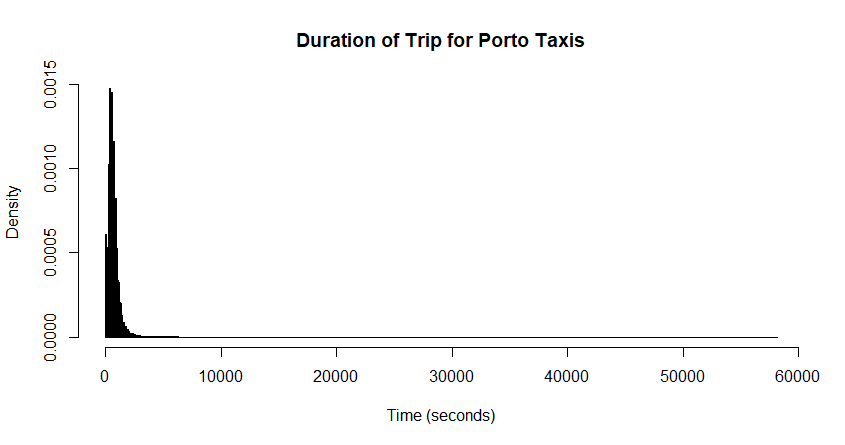
\includegraphics[width=10cm]{B1Hist0.png}
    \caption{Histogram 1 of Trip Time (breaks = 2000)}
    \label{fig:b1histo0}
    \end{figure}
    Upon seeing this histogram of our trip duration we noticed that the scale of the x-axis was unneccesarily large. The maximum trip duration in our data set was 58200 seconds, which equates to a 16 hour taxi trip! In order to find a well-fitting density function, we decided via inspection to rule out values over 6000 seconds (Approximately 3400 of our 1.7 million values). This gave us a histogram following what appeared to be a gamma distribution, so we calculated our $r_{est}$ and $\lambda_{est}$ accordingly:
    \begin{equation}
         r_{est} = \frac{{M_1}^2}{s^2} \;\;\;\; \lambda_{est} = \frac{M_1}{s^2} 
    \end{equation}
    Where $M_1$ is our sample mean and $s^2$ is our variance.
    \\\\
    \begin{figure}[H]
    \centering
    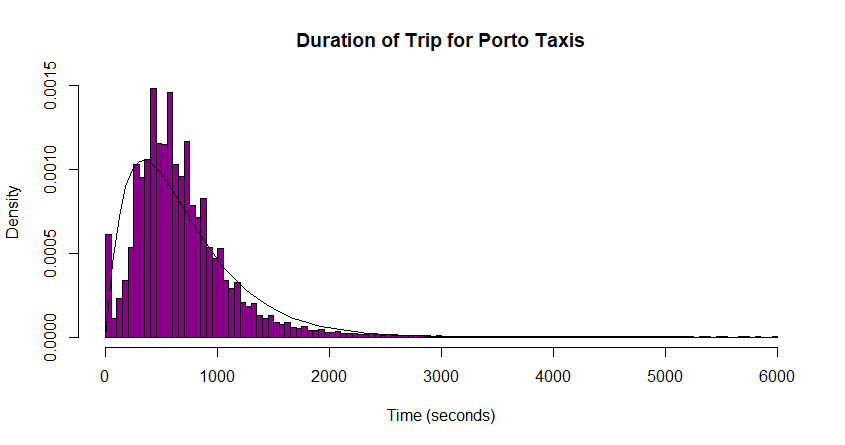
\includegraphics[width=10cm]{B1HistoCurve2.png}
    \caption{Histogram and density curve estimate of Trip Time (breaks = 200) $r_{est} \approx 1.9612$ and $\lambda_{est} \approx 0.002809$ }
    \label{fig:b1histo1}
    \end{figure}
    
    This density curve we found fits our curve pretty well, but below 400 it overestimates and between 400 seconds and 1000 it underestimates. Something that was of interest was the spike in trip times around 0. Upon further inquiry we found that there were 36,510 trips that had a duration of 0 seconds. This is most likely due to the way we handled POLYLINE when there was only one coordinate pair. To remedy this issue we found it reasonable to omit values where the trip time was 0 seconds for the sake of finding a model that fits the majority of our data better. Our resulting histogram and density curve looked like this: 
    
    \begin{figure}[H]
    \centering
    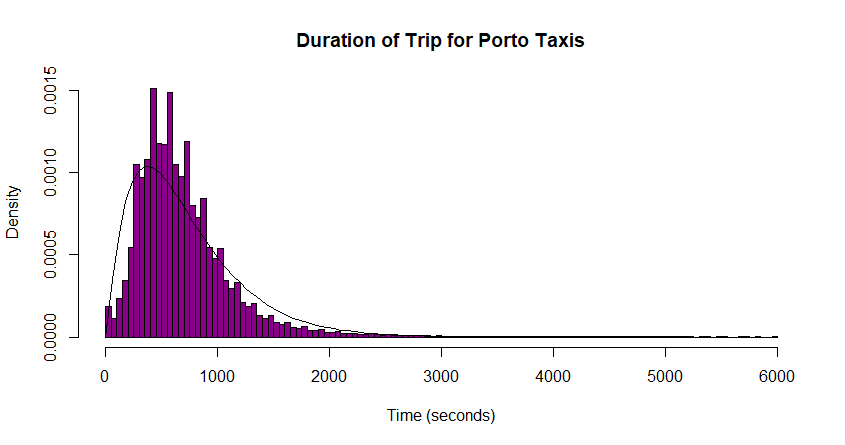
\includegraphics[width=10cm]{B1HistoCurve3.png}
    \caption{Histogram and density curve estimate of Trip Time (breaks = 200) $r_{est} \approx 2.0938$ and $\lambda_{est} \approx 0.002935$ }
    \label{fig:b1histo1}
    \end{figure}
    
    This density curve fit our histogram better than the last to a marginal degree. Although the density function doesn't match our data perfectly, we can conclude that $f_t$ can be modeled by a gamma distribution with $r_{est} \approx 2.0938$ and $\lambda_{est} \approx 0.002935$ .
    
    \item Explore finding a model for $f_B$ from one of our density families.
    \\
    \\To get the busy rate, we needed to first find both the total time and the busy time; in other words, we had to build a model for the drivers' behavior routine.
    \\Our first hypothetical model is that the driver started his/her day with the first trip and ended the day with the last trip. The total time of each driver is calculated as:
    \begin{equation}
        \sum(end\_time - start\_time + last\_trip\_time)
    \end{equation}$ $ and the busy time is $\sum trip\_time$
    \\Our code is the function of getTotalTimeRate in ProbB\_2.R.(note that the result of our function had its first row to be all NAs and we had to get rid of them)
    \begin{lstlisting}

m <- getTotalTimeRate(train)
hist(m[(2:dim(m)),4],
       main="Time Proportion of being busy for Porto Taxis" ,
       xlab="Rate (from 0 to 1)",
       ylab =  "frequency" ,
       breaks = 20,
      freq=FALSE
  )
    \end{lstlisting}
    Several problems might occur from this assumption. First, if the drivers just did one trip on a day and/or had relatively short time between trips, the actual time spent waiting would be highly ignored. Moreover, if the driver was used to resting in daytime and working during night, our model would just add the whole day into the total time.
    \\Unfortunatly, the graph from this assumption showed almost 100\% of being totally busy:
    \begin{figure}[H]
    \centering
    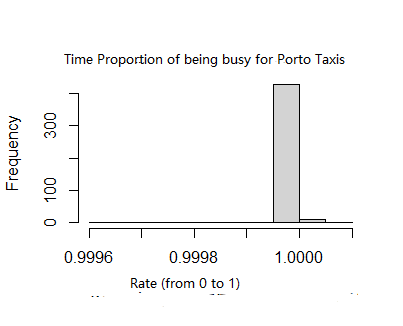
\includegraphics[width=8cm]{B2Hist1.jpg}
    \caption{Histogram 1 for Busy Rate }
    \label{fig:b2hist1}
    \end{figure}
    From the graph we could conclude that almost every driver just did single trip per day and/or had almost no interval between each assigned trip. This proved that our assumption would be invalid for this data set.
    \\
    \\So we came up another hypothetical model: we record the earliest and last time a driver's ID occurs and get the difference of the two plus the time of his/her last trip time 
    \\Our new code was the function getTrueTotalTimeRate in the same file.(note that the result of our function had its first row to be all NAs and we had to get rid of them)
    \begin{lstlisting}

m <- getTrueTotalTimeRate(train)
hist(m[(2:dim(m)),4],
       main="Time Proportion of being busy for Porto Taxis" ,
       xlab="rate (from 0 to 1)",
       ylab =  "density" ,
       breaks = 20,
      freq=FALSE
  )
    \end{lstlisting}
    This assumption's problem was that the total time might be calculated too large. Once a driver did trips with long intervals, like he/she drove once a year, the error would be huge since the calculated total was much greater than the actual time for waiting.
    \\Fortunately, the distribution graph of this hypothetical model was:\begin{figure}[H]
    \centering
    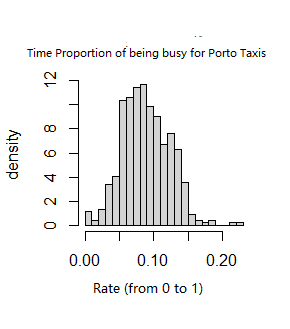
\includegraphics[width=8cm]{B2Hist2.png}
    \caption{Histogram 2 of Bust Rate (breaks = 20)}
    \label{fig:b2hist2}
    \end{figure}
   Looking at the histogram, we notice the x-values in this graph can only possibly range from $[0,1]$. We also notice that the general shape of the graph looks like a beta distribution. Therefore we calculated our $\alpha$ and $\beta$ parameters as such: 
   \begin{equation}
    \alpha = ( (1-\mu)/\sigma^2- 1/\mu)\cdot \mu^2 \;\;\;\;\;\;\;\;
    \beta = \alpha (1/\mu -1)
   \end{equation}
   \begin{lstlisting}
     > mean(m[,4],na.rm = TRUE)
    [1] 0.0888136
    > var(m[,4],na.rm = TRUE)
    [1] 0.0011547
   \end{lstlisting}
    $\mu \approx  0.0888136$ and $\sigma^2 \approx 0.0011547$ 
   \\ $\alpha = ( (1-\mu)/\sigma^2- 1/\mu)* \mu^2 \approx 6.135579$
   \\ $\beta = \alpha (1/\mu -1) \approx 62.9482$
   \begin{lstlisting} 
   p <- seq(0,1,0.001)
   lines(p, dbeta(p, 6.135579, 62.9482), col=2)
   \end{lstlisting}
   And the graph was
   \begin{figure}[H]
    \centering
    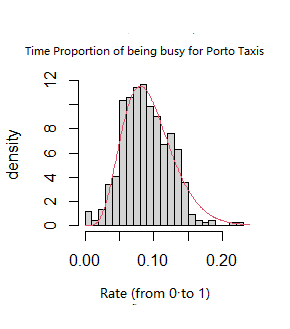
\includegraphics[width=8cm]{B2Hist2Curve1.png}
    \caption{Histogram 3 of Busy Rate (breaks = 20)}
    \label{fig:b2hist2}
    \end{figure}
    This curve fits our histogram quite well. Although there are intervals which our curve overestimates and underestimates our histogram, we can still reasonably conclude that $f_B$ be modeled by a beta distribution with $\alpha \approx 6.135579$ and $\beta \approx  62.9482$
    \item Investigate whether the type of call used to summon the taxi makes much difference in mean trip time.
    \\To figure out whether the trip time was affected by the call type, we first pick the trips and stored them in a data frame called m2 with its 3 columns to store the trip time of A, B or C call type. 
    \begin{lstlisting}> 
mean(m2$a,na.rm = TRUE)
[1] 750.3380
mean(m2$b,na.rm = TRUE)
[1] 665.1738
mean(m2$c,na.rm = TRUE)
[1] 772.3879
var(m2$a,na.rm = TRUE)
[1] 260131.5
var(m2$b,na.rm = TRUE)
[1] 233124
var(m2$c,na.rm = TRUE)
[1] 970286.5
    \end{lstlisting}
    From the data above, now we can calculate the p-values and confidence interval to find out whether the mean times were affected or not. In response to the task's request, we chose to actually compare the data of one call type and the means of 2 other.
    \\
    \\Using t.test(m2[1], mu = 665.1738, alternative = "two.sided")
    \\we got p-value between A \& mean(B) \textless 2.2e-16
    \\Using t.test(m2[1], mu = 772.3879, alternative = "two.sided")
    \\we got p-value between A \& mean(C) \textless 2.2e-16
    \\Using t.test(m2[2], mu = 750.3380, alternative = "two.sided")
    \\we got p-value between B \& mean(A) \textless 2.2e-16
    \\Using t.test(m2[2], mu = 772.3879, alternative = "two.sided")
    \\we got p-value between B \& mean(C) \textless 2.2e-16
    \\Using t.test(m2[3], mu = 750.3380, alternative = "two.sided")
    \\we got p-value between C \& mean(A) \textless 2.2e-16
    \\Using t.test(m2[3], mu = 665.1738, alternative = "two.sided")
    \\we got p-value between C \& mean(B) \textless 2.2e-16
    \\
    \\Our $H_0$ is that the trip times were not affected by call type. Since the p-values were much too small, we could say that the null hypothesis was powerfully rejected and the statistical results supported that the call type would hugely affect the mean time of trips. The reason why the p-values were so small could come from the huge sample size in this case.
    \\
    \\Also, we can get the 95\% confidence intervals as:
    \\Calltype A = (748.6828,751.9931)    
    \\Calltype B = (664.1274,666.2202)    
    \\Calltype C = (769.7310,775.0448)
    \\And we could see from these intervals that each set had their intervals very stable and far from each other.
    \\
    \\Just for verification, we also performed t-tests upon each pairs directly:  
    \begin{lstlisting}
    t.test(m2[1],m2[2])

    Welch Two Sample t-test

data:  m2[1] and m2[2]
t = 85.242, df = 667101, p-value < 2.2e-16
alternative hypothesis: true difference in means is not equal to 0
95 percent confidence interval:
 83.20605 87.12240
sample estimates:
mean of x mean of y 
 750.3380  665.1738 

t.test(m2[1],m2[3])

    Welch Two Sample t-test

data:  m2[1] and m2[3]
t = -13.806, df = 835272, p-value < 2.2e-16
alternative hypothesis: true difference in means is not equal to 0
95 percent confidence interval:
 -25.18020 -18.91967
sample estimates:
mean of x mean of y 
 750.3380  772.3879 

t.test(m2[2],m2[3])

    Welch Two Sample t-test

data:  m2[2] and m2[3]
t = -73.589, df = 693750, p-value < 2.2e-16
alternative hypothesis: true difference in means is not equal to 0
95 percent confidence interval:
 -110.0697 -104.3586
sample estimates:
mean of x mean of y 
 665.1738  772.3879
    \end{lstlisting}
    And we could see from each t-test the 2 sets are obviously different from each other. 
    \\In conclusion, our findings indicate that average trip time could be highly affected by the call type; specifically, type A would bound the time close to 750.3380 seconds, type B would bound the time close to 665.1738 seconds, and type C would bound the time close to 772.3879 seconds.
    \\
    \\\item  Develop models for predicting trip time from other variables.
\end{enumerate}

\textbf{General Method}
\\
\\We predicted trip time from these variables: (1) Trip Distance and (2) Time of Day
For each of the three mentioned variables, we tested all of our models (three linear and two ML) against these variables. 
\\
\\
Trip Distance and Time of Day were not given in the original data set. Therefore, we used given columns to generate these two variables using the following methods: 
\\
\\Trip Distance was calculated from our previously vectorized POLYLINE. Wherever rows contained the value "True" in the given column "MISSING DATA", those rows were excluded from the final dataset. For each pair of adjacent coordinates, we calculated the distance in Kilometers (km) using the Haversine formula. In special cases where the POLYLINE vector only contained one pair of coordinates, we made the assumption that the person traveled 0 km.  
\begin{lstlisting}
#calculate the distance
    dis <- 0
    if(missing[i] == "False") { #change this depending on the dataset, FALSE if using test data, False if using big data
      if (length(x) >= 4) {
        for(j in seq(from=1, to=(length(x)-3), by =2)) {

          #We perform the Haversine formula to calculate the spherical distance between the two coordinates.
          rad <- pi/180
          a <- x[j]rad
          b <- x[j+2]rad
          lat <- (x[j+3]rad) - (x[j+1]rad)
          lon <- b - a
          hav <- (sin(lat/2))^2 + cos(a)cos(b)(sin(lon/2))^2
          rsine <- 2atan2(sqrt(hav), sqrt(1 - hav))
          d <- 6378.137*rsine
          dis <- dis + d
        }
      distance[i] <- dis
      } else {
        distance[i] <- 0 #The person spent less than 15 seconds in the car, assume distance traveled is 0
      }
    } else {
      distance[i] <- NA
      }
  }
  tripdata <- data.frame(tripID,tripTime,distance)
  return(tripdata)
\end{lstlisting}
Time of Day was calculated based on the given "TIMESTAMP" column, which gives the start time of the taxi trip in UNIX time. To convert the UNIX time to a more useable time value, we ran each row of TIMESTAMP on this line of code:
\begin{lstlisting}
timeofday <- dataset$TIMESTAMP %% 86400
\end{lstlisting}
The result is a value that, irrespective of the day, represents a time relative to the start of the day; a greater value indicates a later time of day whereas a smaller value closer to zero indicates a time closer to the start of the day (midnight of that day).
\\
\\
\textbf{General Overview of Models}
\\
\\For linear models, we used linear regression, polynomial regression where deg=2, and polynomial regression where deg=4. We expect linear regression and polynomial regression to the 2nd degree to perform fairly well. 
\\
\\The amount of time you spend driving likely scales linearly to how far you drive (trip distance). However, in the case of heavy traffic, polynomial regression may make more sense, where trip time may grow exponentially based on not only how far the taxi ride is, but how much traffic there is along the path. At certain times of day, trip time could increase exponentially during periods of heavy traffic, such as common work hours (i.e 9AM - 5PM). 
\\
\\Both Random Forest (RF) and K Nearest Neighbors (KNN) were chosen as our ML models. KNN does not make any assumptions on the data distribution, so it is a good contrast to the parametric models we previously chose, which do make assumptions on the data distribution. RF was simply chosen as it was one of the more intuitive models to choose from. 


\textbf{Linear Models}
\\
\\For each of our three linear models, we performed three function calls using (1) trip distance (pdist), (2) time of day (ptimeday), (3) both trip distance and time of day (pdisttimeday). For our holdout set, we chose 400,000, which is roughly 20\% of the overall dataset. 
\\
\\The polynomial regression models were called the same. They are named as follows, where $n$ is the degree of the model: (1) trip distance (poly$n$dist), (2) time of day (poly$n$timeday), (3) both trip distance and time of day (poly$n$disttimeday)

\begin{lstlisting}
#linear 
lindist <- qeLin(pdist, 'time', holdout = 400000)
lintimeday <- qeLin(ptimeday, 'time', holdout = 400000)
lindistimeday <- qeLin(pdistimeday, 'time', holdout = 400000)

#polynomial degree 2 
poly2dist <- qePolyLin(pdist, 'time', deg = 2 holdout = 400000)      
poly2timeday <- qePolyLin(ptimeday, 'time', deg = 2 holdout = 400000)        
poly2distimeday <- qePolyLin(pdistimeday, 'time', deg = 2 holdout = 400000)   

#polynomial degree 4
poly4dist <- qePolyLin(pdist, 'time', deg = 4 holdout = 400000)
poly4timeday <- qePolyLin(ptimeday, 'time', deg = 4 holdout = 400000)
poly4distimeday <- qePolyLin(pdistimeday, 'time', deg = 4 holdout = 400000)
\end{lstlisting}

The testing accuracies in seconds and $R^2$ values for each are as follows: 
\begin{center}
 \begin{tabular}{||c || c c c||} 
 \hline
  \multicolumn{4}{|c|}{Testing Accuracies for Linear Models} \\
  \hline
dataset name & Linear & Polynomial degree=2 & Polynomial degree=4\\ [0.5ex] 
 \hline\hline
 distance only & 240.9367 & 236.0364 & 680.0475\\ 
 \hline
 time of day only & 349.2628 & 368.3578 & 449.6158\\
 \hline
 distance and time of day & 237.8981 & 276.5053 & 405.8638\\ [1ex] 
 \hline
\end{tabular}
\end{center}

\begin{center}
 \begin{tabular}{||c || c||} 
 \hline
 \multicolumn{2}{|c|}{$R^2$ values} \\
  \hline
dataset name & Linear\\ [0.5ex] 
 \hline\hline
 distance only & .4447415\\ 
 \hline
 time of day only & .0008947832\\
 \hline
 distance and time of day & .4491876\\ [1ex] 
 \hline
\end{tabular}
\end{center}
\\
\\
\textbf{Analysis of Linear Model results}
\\
\\Our testing accuracies for the linear and Polynomial degree=2 models performed much better than 
Polynomial degree=4. This makes sense, as the polynomial degree=4 shape is likely over-fitting the data, and does not generalize very well. While the model captures the fit of the training data well, it likely performs poorly on the holdout set of 400,000 rows. The time of day variable testing accuracy generally seemed to be worse compared to distance; this makes sense, as time of day does not necessarily have any bearing on the trip distance aside from the moments in the day when there is high traffic. Using trip distance is much more reliable, as longer distances will always take more time to travel across. 

\\The $R^2$ values involving the distance variable seem pretty standard. What is concerning is the $R^2$ value for time of day is incredibly low, further indicating that the time of day likely does not have a direct effect on the trip time. 
\\
\\
\textbf{Constructing a 95\% Confidence Interval of $E(Y|X=u)$}
\\ 
\\ In the expression $E(Y|X=u)$, Y is the outcome we are predicting and X is the set of columns we wish to predict Y from. Our Y in this case is trip time and X is either distance, time of day, or both. In order to find the $E(Y|X=u)$we called the function predict.lm() upon our linear models in the console:
\begin{lstlisting}
preddist <- .lm(lindist, cdist, interval = "confidence")
predtimeday <- predict.lm(lintimeday, ctimeday, interval = "confidence")
preddistimeday <- predict.lm(lindistimeday, cdistimeday, interval = "confidence")
\end{lstlisting}
In the function call, cdist, ctimeday, and cdistimeday were our datasets used to find our linear models not including the time column (In other words, our X). The function used these values to pass into our linear model as values to predict the time from. By default this function finds a confidence interval of 95\%. These functions each returned a 3 column matrix labeled fit, lower bound, and upper bound with 1.7 million rows of confidence intervals for predicting time from the data we input. These essentially found $Y|X=u$, so in order to find the expected value we just needed to calculate the mean of each column. Our resulting expected value confidence intervals are in the table below: 

\begin{center}
 \begin{tabular}{||c || c c c||} 
 \hline
  \multicolumn{4}{|c|}{95\% Confidence Interval} \\
  \hline
dataset name & fit & lower bound & upper bound\\ [0.5ex] 
 \hline\hline
 distance only & 716.3175 & 715.2997 & 717.3353\\ 
 \hline
 time of day only & 716.2838 & 714.6757 & 717.892\\
 \hline
 distance and time of day & 716.5103 & 715.1909 & 717.8297\\ [1ex] 
 \hline
\end{tabular}
\end{center}
These values show that we are 95\% confident that the true mean trip time lies within the interval (715.2997, 717.3353) for the linear model where X = distance; for X = time of day, we are 95\% confident that the true mean trip time lies within the interval (714.6757, 717.892); for X=distance and time of day we are  95\% confident that the true mean trip time lies within the interval (715.1909, 717.8297).
\\\\
Our true mean trip time was 716.4265 for our X that we used, which is reflected in our confidence intervals well.
\\\\
The narrow width of each of the three confidence intervals can be explained by our large n value of 1.7 million rows; as n grows in size, the precision of the interval increases.
\\
The slightly wider confidence interval for the linear model where X = time of day is consistent with the poor testing accuracy and low $R^2$ values we found. It seems however, that the width of the interval is still narrow due to the sheer size of the dataset. 
\\
\\\textbf{Machine Learning Models} 
\\
\\We used KNN and RF models to predict trip time based on (1) Trip Distance (knndist, prfdist), (2) Trip Time of day (knntimeday, prftimeday), (3) both trip distance and time of day (knndistimeday, prfdistimeday). We used the same number of rows (400,000) for the holdout set as the linear models. \\
\\For k, we chose an arbitrary value of 100 due to computing restraints. 
\\
\\For the creation of random trees models we created datasets prfdist, prftimeday, and prfdistimeday. Each dataset is a randomly sampled subset of pdist, ptimeday, and pdistimeday of size 10000. This limit of size 10000 was introduced due to how expensive the random tree computations are. 

\begin{lstlisting}
#KNN 
knndist <- qeKNN(pdist, 'time', 100, holdout = 400000)
knntimeday <- qeKNN(ptimeday, 'time', 100, holdout = 400000)
knndistimeday <- qeKNN(pdistimeday, 'time', 100, holdout = 400000)

#RF 
rfdist <- qeRF(prfdist, 'time')
rftimeday <- qeRF(prftimeday, 'time')
rfdistimeday <- qeRF(prfdistimeday, 'time')
\end{lstlisting}
We then examined the testing accuracy each model gave to assess the effectiveness in predicting trip time. The testing accuracies in seconds for each model are as follows: 
\begin{center}
 \begin{tabular}{||c || c c ||} 
 \hline
 \multicolumn{3}{|c|}{Testing Accuracies for Machine Learning Models} \\
  \hline
dataset name & KNN & RF\\ [0.5ex] 
 \hline\hline
 distance only & 221.7606 & 258.344\\ 
 \hline
 time of day only & 350.3027 & 405.9462\\
 \hline
 distance and time of day & 207.2447 & 203.7757\\ [1ex] 
 \hline
\end{tabular}
\end{center}

\\Testing accuracy seems to be lowest with both distance and time of day, while time of day has by far the worst testing accuracy. The higher testing accuracy for both distance and time of day leads us to believe that perhaps both variables together likely could indicate how long a trip will take. For example, a trip at 5pm across 50 miles will certainly take longer than a trip at 1am across 3 miles. Meanwhile, a trip at 1am across 50 miles could take a similar amount of time as a trip across 3 miles at 5pm; the additional information of time of day in conjunction with trip distance likely leads to better prediction. 


\begin{figure}[H]
    \centering
    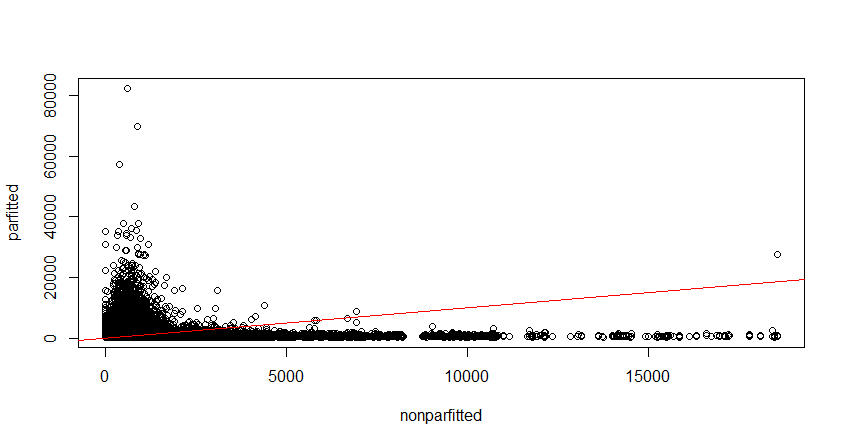
\includegraphics[width=12cm]{lindistvsknndist.png}
    \caption{linear model distance only vs KNN distance only}
    \label{fig:b2hist2}
    \end{figure}
\begin{figure}[H]
    \centering
    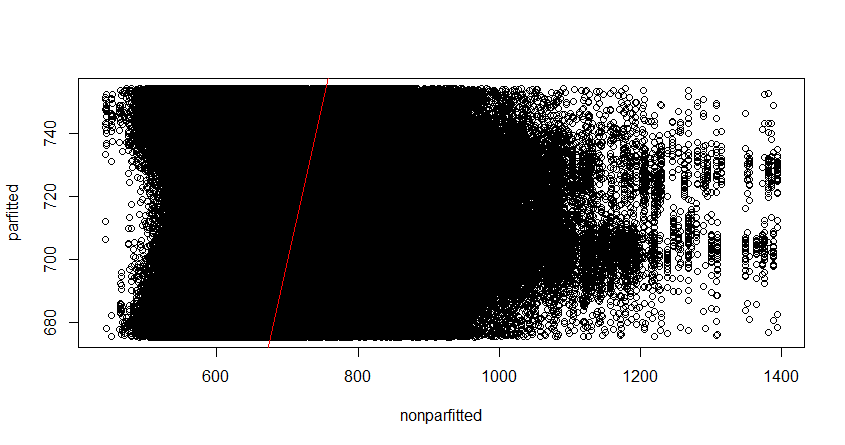
\includegraphics[width=12cm]{lintimedayvssknntimeday.png}
    \caption{linear model time of day only vs KNN time of day only}
    \label{fig:b2hist2}
    \end{figure}

\begin{figure}[H]
    \centering
    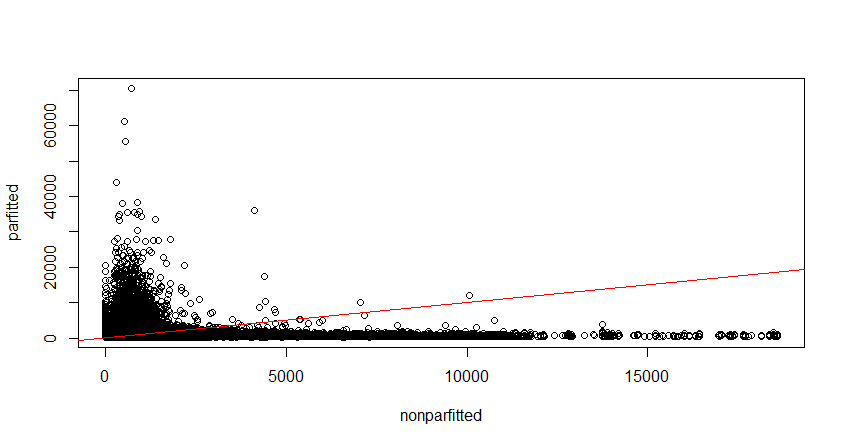
\includegraphics[width=12cm]{lindistimedayvsknndistimeday.png}
    \caption{linear model distance and time of day vs KNN distance and time of day}
    \label{fig:b2hist2}
    \end{figure}
    
\\
\\\textbf{Linear Models vs KNN}
\\
\\The three plots shown above compare each of the three linear models to each of the KNN models, for their respective dataset (i.e distance only linear vs distance only KNN). The plot has the KNN values on the x-axis and the linear model values on the y-axis. The plot assumes the KNN values to be correct, and is measuring the performance of the linear model, which assumes the distribution of the data to be linear. 
\\
\\The plots involving the distance variable (Figures 7 and 9) both seem to cluster above the y=x red line from around x=0 to x=3000. This is an indication that our linear model is over-predicting trip time for lower values. For x greater than 3000, the model seems to under-predict trip time.  
\\
\\The plot for time of day is all over the place, and no real meaningful conclusion can be drawn from this plot. This, however, is consistent with our low $R^2$ value, further indicating that trip time of day alone is not a good predictor of trip duration. 
\\
\\Overall, the Machine Learning models did seem to do a better job at prediction, as both KNN and RF generally produced better prediction accuracies. However, the performance was marginally better. Trip distance does seem to be a good predictor of trip duration, while trip time of day alone seems to bear no meaning to the trip duration. 
\\
\\\textbf{Further Research}
\\
\\For further research, it would be interesting to see how other variables could be used to predict trip duration, such as trip location, which could be calculated based on regions throughout the area from the given POLYLINE coordinates. It would also be interesting to see how different k values perform with our KNN model, with larger values of k that better reflect the large dataset size. 
\\

\appendix
\section{Appendices}
\subsection{Individual Contributions}
\\ What each team member contributed to the project. \\
\textbf{Team Member: } Alan Wu \\
Initial Histograms for task 1, initial method for finding proportion of time driver was busy for task 2, code for task 3, written analysis for task 4 
\\
\textbf{Team Member: } Joshua Winter \\
Coding of trip duration and trip distance calculations for task 1 and 4; data analysis for task 1; separated the trip times by call type in task 3; data cleaning, creation, management, computations, and graphs for task 4. 
\\
\textbf{Team Member: } Dongyu  Chen \\
Coding of finding the second theoretical and usable method of rates and building the model, construction of all the histograms and  analysis for the data for task 2; coding of finding the time of each type, t-tests, computation, and statistically analysis for task 3; and organization and analysis for task 4.
\\
\textbf{Team Member: } Rishabh  Manu \\
Testing and bug fixing of code in  problems 1 and 2. Coding and developing models for Machine Learning methods in problem 4. Bug fixing for different issues code for problem 4. Analyzing results of linear regression summary. Creating/coding 95 percent confidence interval from linear regression.
\\
\subsection{Code}
\begin{lstlisting}
#This function was used to create vectors of distance and time for each row in the dataset
findTripData <- function(dataset) {
  
  ppoly <- unlist(dataset$POLYLINE)
  ID <- unlist(dataset$TRIP_ID)
  missing <- unlist(dataset$MISSING_DATA)
  # initialize our data frame to store the time and distance of each unique trip
  
  tripID <- vector("numeric", length = length(ID))
  tripTime <- vector("numeric", length = length(ppoly))
  distance <- vector("numeric", length = length(ppoly))
  
  # iterate through each trip and calculate time and distance
  for(i in 1:length(ppoly)) {
    tripID[i] <- ID[i]
    p <- ppoly[i]
    
    if(i%%10000 == 0) { print(i)}
    # turn the polyline string into a vector of coordinate values
    x <- unlist(regmatches(p, gregexpr('\\(?[0-9.]+', p)))
    x <- as.numeric(x)
    if(length(x) <= 2) {
      tripTime[i] <- 0
    }
    else {
      tripTime[i] <- 15*((length(x)-2)/2)
    }
 
    
    #calculate the distance
    dis <- 0
    if(missing[i] == "False") { #change this depending on the dataset, FALSE if using test data, False if using big data
      if (length(x) >= 4) {
        for(j in seq(from=1, to=(length(x)-3), by =2)) {
          
          #We perform the haversine formula to calculate the spherical distance between the two coordinates.
          rad <- pi/180
          a <- x[j]*rad
          b <- x[j+2]*rad
          lat <- (x[j+3]*rad) - (x[j+1]*rad)
          lon <- b - a
          hav <- (sin(lat/2))^2 + cos(a)*cos(b)*(sin(lon/2))^2
          rsine <- 2*atan2(sqrt(hav), sqrt(1 - hav))
          d <- 6378.137*rsine
          dis <- dis + d
        }
      distance[i] <- dis
      } else {
        distance[i] <- 0 #The person spent less than 15 seconds in the car, assume distance traveled is 0
      }
    } else {
      distance[i] <- NA
      }
  }
  tripdata <- data.frame(tripID,tripTime,distance)
  return(tripdata)
}

library("data.table")

processPolyHelper2 <- function(p)
{ 
  x <- unlist(regmatches(p, gregexpr('\\(?[0-9.]+', p)))

  sum = 15*(length(x)-2)/2
  if(length(x) <= 3){
    return(0)
  }else{
  return(sum)
  }
  
}


 # This function was used to get the total time calculated from the time interval between a driver's first and last trips everyday plus the last trip time every day. It also calculated the total trip time and thus gets the time rate of this version.
getTotalTimeRate <- function(p){
  #sort the data set for calculation based on id and time
  poly1 <- p[order(p$TIMESTAMP),]
  poly2 <- poly1[order(poly1$TAXI_ID),]
  
  baseID <- poly2$TAXI_ID[1]
  baseTime <- poly2$TIMESTAMP[1]
  baseTotalTime <- 0
  baseRunTime <- processPolyHelper2(poly2$POLYLINE[1]) 
  storedTime <- poly2$TIMESTAMP[1]
  m <- matrix(ncol=4)
  colnames(m) <- c('TAXI_ID', 'TotalTime', 'TotalRunTime','Rate')
  
  for (i in 2:length(poly2$TIMESTAMP)) {
    
    if(poly2$TAXI_ID[i] == baseID ){
      if(as.IDate(poly2$TIMESTAMP[i]) == as.IDate(baseTime)){
        #same person same day
        #store the time of last run
        storedTime <- poly2$TIMESTAMP[i]
        #add run time
        baseRunTime <- baseRunTime + processPolyHelper2(poly2$POLYLINE[i])
        
      }
      else{
        #same person different day
        #add total time before
        baseTotalTime <- baseTotalTime + storedTime - baseTime + processPolyHelper2(poly2$POLYLINE[i-1])
        #add run time
        baseRunTime <- baseRunTime + processPolyHelper2(poly2$POLYLINE[i])
        #change both first and last time (or at least so far) of the day
        storedTime <- poly2$TIMESTAMP[i]
        baseTime <- poly2$TIMESTAMP[i]
      }
      
    }else{
      #differ person
      #add the last total time
      baseTotalTime <- baseTotalTime + storedTime - baseTime + processPolyHelper2(poly2$POLYLINE[i-1])
      
      
      #insert(m,c(baseID,baseTotalTime,baseRunTime,baseRunTime/baseTotalTime))
      m <- rbind(m,c(baseID,baseTotalTime,baseRunTime,baseRunTime/baseTotalTime))
      
      #reset all
      baseTotalTime <- 0
      baseRunTime <- processPolyHelper2(poly2$POLYLINE[i])
      
      baseID <- poly2$TAXI_ID[i]
      storedTime <- poly2$TIMESTAMP[i]
      baseTime <- poly2$TIMESTAMP[i]
    }
    
    if(i == length(poly2) ){
      #last line
      #add last total time
      storedTime <- poly2$TIMESTAMP[i]
      baseTotalTime <- baseTotalTime + storedTime - baseTime + processPolyHelper2(poly2$POLYLINE[i])
      #insert (baseID,baseTotalTime,baseRunTime,baseRunTime/baseTotalTime))
      m <- rbind(m,c(baseID,baseTotalTime,baseRunTime,baseRunTime/baseTotalTime))
      
    }
  }
  
  
  
  return(m)
  
}
 # This function was used to get the total time calculated from the time interval between a driver's first and last trips in the total record plus the last trip time. It also calculated the total trip time and thus gets the time rate of this version.
getTrueTotalTimeRate <- function(p){
  #sort the data set for calculation based on id and time
  poly1 <- p[order(p$TIMESTAMP),]
  poly2 <- poly1[order(poly1$TAXI_ID),]
  
  baseID <- poly2$TAXI_ID[1]
  baseTime <- poly2$TIMESTAMP[1]
  baseTotalTime <- 0
  baseRunTime <- processPolyHelper2(poly2$POLYLINE[1]) 
  storedTime <- poly2$TIMESTAMP[1]
  m <- matrix(ncol=4)
  colnames(m) <- c('TAXI_ID', 'TotalTime', 'TotalRunTime','Rate')
  
  for (i in 2:length(poly2$TIMESTAMP)) {
    
    if(poly2$TAXI_ID[i] == baseID ){
      
        #same person 
        storedTime <- poly2$TIMESTAMP[i]
        
        baseRunTime <- baseRunTime + processPolyHelper2(poly2$POLYLINE[i])

      
    }else{
      #differ person
      
      baseTotalTime <-  storedTime - baseTime + processPolyHelper2(poly2$POLYLINE[i-1])
      
      
      #insert(m,c(baseID,baseTotalTime,baseRunTime,baseRunTime/baseTotalTime))
      m <- rbind(m,c(baseID,baseTotalTime,baseRunTime,baseRunTime/baseTotalTime))
      
      #reset all
      baseTotalTime <- 0
      baseRunTime <- processPolyHelper2(poly2$POLYLINE[i])
      
      baseID <- poly2$TAXI_ID[i]
      storedTime <- poly2$TIMESTAMP[i]
      baseTime <- poly2$TIMESTAMP[i]
    }
    
    if(i == length(poly2) ){
      #last line
      #add last total time
      storedTime <- poly2$TIMESTAMP[i]
      baseTotalTime <- storedTime - baseTime + processPolyHelper2(poly2$POLYLINE[i])
      #insert (baseID,baseTotalTime,baseRunTime,baseRunTime/baseTotalTime))
      m <- rbind(m,c(baseID,baseTotalTime,baseRunTime,baseRunTime/baseTotalTime))
      
    }
  }
  return(m)
  
}

# This function was used to separate trip duration based on call types. 
separateCallType <- function(p)
{
  calls <- unlist(p$CALL_TYPE)
  times <- unlist(p$time)
  a <- vector("numeric", length(p$CALL_TYPE))
  b <- vector("numeric", length(p$CALL_TYPE))
  c <- vector("numeric", length(p$CALL_TYPE))
  for(i in 1:length(calls))
  {
    if(calls[i] == "A")
    {
      a[i] = times[i] 
    }
    else {
      a[i] = NA
    }
    if (calls[i] == "B") {
      b[i] = times[i]
    }
    else {
      b[i] = NA
    }
    if (calls[i] == "C") {
      c[i] = times[i]
    }
    else {
        c[i] = NA
    }
    if(i%%10000 == 0) { print(i)}
  }
  return(data.frame(a,b,c))
}
\end{lstlisting}
\end{document}
